\section{Das Reziproke Gitter und die Kristallstrukturanalyse}
\subsection{Grundlegende Ideen zur Strukturanalyse}
	Die Gitterkonstanten in Festkörpern liegen zwischen \SI{0,1}{\nano \meter} und \SI{1}{\nano \meter}, wodurch zum Ermitteln der räumlichen Struktur ein einfaches 'Anschauen' wie bspw. unter einem Mikroskop nicht möglich ist. 
	Stattdessen erfolgt die Strukturanalyse von Feststoffen mit Röntgenstrahlung und durch Beschuss mit hochenergetischen Teilchen (beachte Welle-Teilchen-Dualismus). 
	Da diese Teilchen als Informationsträger agieren, werden sie als Sonden bezeichnet. 
	Die Vorraussetzungen an mögliche Sonden lassen sich in zwei Punkten zusammenfassen:
	\begin{enumerate}
		\item Die Sonden müssen mit den Festkörperbausteinen, also den Atomen, bemerkbar wechselwirken.
		\item Eine ausreichend hohe Auflösung muss möglich sein. Dazu muss die charakteristische Wellenlänge der Sonde ähnlich groß sein wie die Gitterkonstante.
	\end{enumerate}

	Mögliche Sonden sind somit
	\begin{itemize}
		\item Photonen wegen ihrer elektromagnetischen Wechselwirkungen mit den Elektronen der Atome,
		\item Elektronen wegen ihrer Coulomb-Wechselwirkung mit den Elektronenhüllen,
		\item Neutronen wegen ihrer Wechselwirkungen mit den Kernen und den magnetischen Momenten der Atome.
	\end{itemize}

	Wichtige Beziehungen und Grö{\ss}en zur Betrachtung der Struktur sind die Energie eines Quantenobjekts
	\begin{equation}
		\label{eq:II.3.1}
		E = \mathrm{h} \nu = \hbar  \omega,
	\end{equation}
	die Wellenzahl
	\setcounter{equation}{3}
	\begin{equation}
		\label{eq:II.3.4}
		\big| \Vec{k} \big| = \frac{2\pi}{\lambda} = \frac{\omega}{c}
	\end{equation}	
	mit
	\stepcounter{equation}
	\begin{equation*}
		\Vec{k} = \big| \Vec{k} \big| \Vec{s} = \frac{2\pi}{\lambda} \Vec{s}
	\end{equation*}
	und der Impuls
	\begin{equation}
		\label{eq:II.3.6}
		\Vec{p} = \hbar \Vec{k}.
	\end{equation}
	$\vec s$ ist der Einheitsvektor in Ausbreitungsrichtung der Strahlung.

	Photonen werden im Bereich der Röntgenstrahlung verwendet, damit die Wellenlängen von \SI{0,01}{\nano \meter} bis \SI{1}{\nano\meter} im Bereich der Gitterkonstante sind. 
	
	Elektronen und Neutronen haben jeweils die Energie
	$$
	E = \frac{p^2}{2m}.
	$$ 
	Mit Gleichung \eqref{eq:II.3.6} folgt
	$$
	E = \frac{\hbar ^2 k^2}{2m}.
	$$
	\stepcounter{equation}
	Mit \eqref{eq:II.3.4} folgt die Wellenlänge der Elektronen
	\begin{equation}
		\label{eq:II.3.8}
		\lambda_{\mathrm{e}^{-}} [\unit{nm}]= \frac{\num{1,2}}{\sqrt{E_{\mathrm{e}^{-}} [\unit{eV}]} }
	\end{equation}
	und der Neutronen
	$$
	\lambda_{\mathrm{Neutronen}} [\unit{nm}] = \frac{\num{0,028}}{\sqrt{E_{\mathrm{N}} [\unit{eV}]} }.
	$$ 
	Um Wellenlängen in der Größenordnung der Gitterkonstanten zu realisieren, müssen Elektronen zwischen \SI{1}{\kilo \electronvolt} und \SI{50}{\kilo \electronvolt} besitzen, Neutronen zwischen \SI{0,01}{\electronvolt} und \SI{0,1}{\electronvolt}.

\subsection{Beugung am Kristallgitter, Lane- und Bragg-Gleichungen}
	Ziel dieses Unterkapitels ist es, die Lage von Beugungsreflexen für periodische Gitterstrukturen herauszufinden. 
	Die Anwendung dieses Wissens erfolgt dann in umgekehrter Reihenfolge: 
	wir bestimmen die Kristallstruktur über experimentell bekannte Lagen von Beugungsreflexen.
	Dazu wird angenommen, dass die Sonden elastisch gestreut werden mit
	\stepcounter{equation}
	\begin{equation}
		\label{eq:II.3.10}
		\omega = \omega', \quad  \big|\Vec{k} \big| =  \big| \Vec{k}' \big|, \quad \Vec{s} \neq \Vec{s}'.
	\end{equation}

\paragraph{Beugung elektromagnetischer Strahlung}
	Bei elektromagnetischer Strahlung wird durch eine einfallende Welle das Elektronensystem in erzwungene Schwingung versetzt.
	Jeder Ort im Festkörper, an dem eine nichtverschwindende Elektronendichte vorliegt, ist dann eine Quelle elektromagnetischer Strahlung.
	\autoref{fig:vl16_abbildung_1} zeigt den groben Versuchsaufbau.

	\begin{figure}[H]
		\centering
		\incfig{vl16_abbildung_1}
		\caption{Schematischer Versuchsaufbau zur Kristallstrukturanalyse mit Photonen im Röntgenbereich. 
			Die Röntgenstrahlung tritt nahezu eben auf die Probe. 
			Die Elektronen im Kristallgitter agieren als Streuzentren und emittieren selber Strahlung.
			Diese wird von einem Detektor aufgenommen.
			Dadurch können Rückschlüsse auf die Struktur des Kristalls getroffen werden.
		}
		\label{fig:vl16_abbildung_1}
	\end{figure}

\paragraph{Richtung abgebeugter Wellen}
	Bei gro{\ss}en Entfernungen werden die gebeugten Wellen als ebene Wellen genähert mit
	\begin{equation}
		\label{eq:II.3.11}
		\Vec{E} (\Vec{r}, t) = \Vec{A} (\hat{\Vec{r}}) e^{i (\Vec{k} \Vec{r} - \omega t)} e^{i \varphi (\hat{r})}.
	\end{equation}
	$\Vec{A} (\hat{\Vec{r}})$ ist ein Amplitudenfaktor, welcher proportional zur Elektronendichte am Streuzentrum ist und $e^{i \varphi(\hat{r})}$ ist ein Phasenfaktor.
	In \autoref{fig:vl16_abbildung_2} werden geometrische Vorüberlegungen zur Streuung dargestellt.

	\begin{figure}[H]
		\centering
		\incfig{vl16_abbildung_2}
		\caption{Geometrische Vorüberlegungen zur Streuung elektromagnetischer Strahlung an zwei Streuzentren (schwarze Punkte).}
		\label{fig:vl16_abbildung_2}
	\end{figure}

	Der Gangunterschied für zwei beliebige Streuzentren ist
	\begin{equation}
		\label{eq:II.3.12}
		\begin{split}
			\Delta g = a - b &= \hat{\Vec{r}} \cdot \Vec{s}\, ' - \hat{\Vec{r}}\cdot  \Vec{s} \\
			&= \hat{\Vec{r}}\cdot\left( \Vec{s} \, ' - \Vec{s} \right) 
		\end{split}
	\end{equation}
	Die Phase zwischen den gestreuten Strahlen ist
	\begin{equation}
		\label{eq:II.3.13}
		\varphi = 2 \pi \frac{\Delta g}{\lambda} = \big| \Vec{k} \big| \Delta g \overset{\ref{eq:II.3.12}}{=} \left( \Vec{k}\,' - \Vec{k} \right)\cdot\hat{\Vec{r}},
	\end{equation}
	also
	\begin{equation}
		\label{eq:II.3.14}
		\varphi(\hat{\Vec{r}}) = \Delta \Vec{k} \cdot \hat{\Vec{r}}.
	\end{equation}
	Am Ort $\Vec{r}$ des Beobachters erhält man nach Integration über Gleichung \eqref{eq:II.3.11} mit $\varphi(\hat{\Vec{r}})$ als charakteristische Phase für jedes Streuzentrum
	\begin{equation}
		\label{eq:II.3.15}
		\Vec{E} (\Vec{r}, t) = \int_{V} \mathrm{d}\hat{\Vec{r}}\cdot \Vec{A}(\hat{\Vec{r}}) e^{i \Vec{k}\cdot\Vec{r} + i \varphi(\hat{\Vec{r}})} e^{-i \omega t}.
	\end{equation}
	Da die Streuintensität $I \sim E E^{*}$ ist, können wir den Term $e^{-i \omega t}$ weglassen. Es müssen folgende Kristalleigenschaften berücksichtigt werden:
	\begin{enumerate}
		\item Die Streuzentren sind streng periodisch verteilt. 
			Unter Verwendung der Translationsvektoren im Gitter (siehe \eqref{eq:II.2.14}) kann der Atomabstand $\hat{\vec r}$ umgeschrieben werden zu
			\begin{equation}
				\label{eq:II.3.16}
				\Vec{R}_{m,n,p} = m \Vec{a} + n \Vec{b} + p \Vec{c}.
			\end{equation}
		\item Die Amplitude $\Vec{A}$ der gestreuten Strahlung ist an allen Bausteinen gleich.
		\item Das gesamte Kristallgitter besteht aus je $Z$ Bausteinen in alle drei Raumrichtungen. Das elektrische Feld am Ort $\vec r$ des Beobachters ist somit
			\stepcounter{equation}
			\begin{equation}
				\label{eq:II.3.18}
				\begin{split}
					\Vec{E}(\Vec{r}, t) &= \Vec{A} e^{i \Vec{k} \Vec{r}} \sum_{m,n,p = 0 }^{Z-1} e^{i \Delta \Vec{k} \Vec{R}_{m,n,p}}  \\
					&=  \Vec{A} e^{i \Vec{k} \Vec{r}} \sum_{m = 0}^{Z-1} e^{ i m \Vec{a} \Delta \Vec{k}} \sum_{n = 0}^{Z-1} e^{i n \Vec{b} \Delta \Vec{k}} \sum_{p = 0}^{Z-1} e^{ip \Vec{c} \Delta \Vec{k}}    \\
				\end{split}
			\end{equation}
	\end{enumerate}

\paragraph{Bemerkung:}
	In Gleichung \eqref{eq:II.3.18} hängen das $\vec E$-Feld und das Volumen mit $| \Vec{E}| \sim Z^3$ zusammen. 
	Bei gleichmäßiger Ausleuchtung nimmt die Feldstärke also linear mit dem Volumen der Probe zu!

\paragraph{Lane Gleichungen}
	Die Maxima des elektrischen Feldes treten auf, wenn alle drei Phasenwinkel ganzzahlige Vielfache von $2\pi$ sind.
	Diese Stellen können mithilfe der Lane Gleichungen berechnet werden.
	\begin{important}
		\textbf{Lane Gleichungen}
		\begin{equation}
			\label{eq:II.3.19}
			\begin{split}
				\Vec{a} \cdot \Delta \Vec{k} &= 2 \pi h \\
				\Vec{b} \cdot \Delta \Vec{k} &= 2 \pi k \\
				\Vec{c} \cdot \Delta \Vec{k} &= 2 \pi l
			\end{split}
		\end{equation} 
	\end{important}
	Die Lane-Indizes $h,k,l$ kennzeichnen die Ordnung des Beugungsmaximums.\\
	
	\begin{minipage}{0.6\linewidth}
		Die Lane Gleichungen beschreiben eine Quantisierung des Anteils des Streuvektros $\Delta k $ jeweils in Richtung des beteiligten primitiven Gittervektors.
		Die möglichen Wellenvektoren der gestreuten Welle liegen somit auf Kegeln um die primitiven Gittervektoren $(\Vec{a}, \Vec{b}, \Vec{c})$.
	\end{minipage}
	\hfill
	\begin{minipage}{0.3\linewidth}
		\centering
		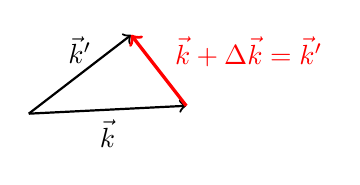
\begin{tikzpicture}
			\draw[thick, ->] (0,0) -- (2,0.1) node[midway, below] {$\vec k$};
			\draw[thick, ->] (0,0) -- (1.3,1) node[midway, above] {$\vec k'$};
			\draw[very thick, color = red, ->] (2,0.1) -- (1.3,1) node[pos = 0.4, anchor = south west] {$\vec k+\Delta\vec k = \vec k'$};
		\end{tikzpicture}
		\captionof{figure}{}
		\label{fig:vl16_abbildung_3}
	\end{minipage}

	Beugungsmaxima treten nur dort auf, wo die Maxima aller drei Beugungsfiguren sich schneiden. 
	Beugungsblder sind also \textbf{Punktbilder}. Mit $I \sim \Vec{E} \Vec{E}^{*}$, Gleichung \eqref{eq:II.3.18} und 
	$$
	\sum_{m=0}^{Z-1}  x^{m} = \frac{1 - x^{Z}}{1 - x}
	$$
	folgt
	\begin{equation}
		\label{eq:II.3.20}
		I \sim A^2 \frac{\sin^2\left( \frac{1}{2} Z \left( \Vec{a} \Delta \Vec{k} \right)  \right) }{\sin^2\left( \frac{1}{2} \Vec{a} \Delta \Vec{k} \right) } \cdot  \frac{\sin^2\left( \frac{1}{2} Z \Vec{b} \Delta \Vec{k} \right) }{\sin^2\left( \frac{1}{2} \Vec{b}\Delta \Vec{k} \right) } \cdot \frac{\sin^2\left( \frac{1}{2} Z \Vec{c} \Delta \Vec{k} \right) }{\sin^2 \left( \frac{1}{2} \Vec{c} \Delta \Vec{k} \right) }
	\end{equation}
	Der Beweis dieses Zusammenhangs ist dem Leser als Übungsaufgabe überlassen. 
	Beobachtbar sind also starke Maxima mit der Breite $\sim \frac{1}{Z}$, da $Z$ sehr groß ist.

\paragraph{Bragg'sche Bedingung} 
	Die Beugung kann als konstruktive Interferenz von Wellen angesehen werden, die von \textbf{Netzebenen} teilweise reflektiert werden. 
	Eine Ebene wird beschrieben durch die Miller-Koordinaten $\left( h,k,l \right)$. 
	Der Abstand zweier benachbarten Ebenen in einem rechtwinkligen Gitter ist
	\begin{equation}
		\label{eq:II.3.21}
		d_{hkl} = \frac{1}{\sqrt{ \frac{h^2}{a^2} + \frac{k^2}{b^2} + \frac{l^2}{c^2}} },
	\end{equation}
	wobei $a,b,c = |\Vec{a}|, |\Vec{b}|, |\Vec{c}|$ die Längen der primitiven Gittervektoren sind. 
	Auch der Beweis dieses Zusammenhangs ist dem Leser überlassen.
	In \autoref{fig:vl16_abbildung_4} werden geometrische Vorüberlegungen zur Aufstellung der Bragg'schen Bedingung getroffen.

	\begin{figure}[H]
		\centering
		\incfig{vl16_abbildung_4}
		\caption{Geometrische Vorüberlegungen zur Reflektion von Strahlung an Netzebenen im Kristallgitter. 
			Es ist $\vartheta = 2\varphi$, wobei $\vartheta$ außerhalb der Probe gemessen werden kann.
		}
		\label{fig:vl16_abbildung_4}
	\end{figure}

	Konstruktive Interferenz für Strahlung der Wellenlänge $\lambda$ erfolgt bei
	$$
	2d_{hkl}  \sin\left( \varphi \right)  = m \lambda.
	$$
	Mit $\vartheta=2\varphi$ folt die 
	\begin{important}
		Bragg'sche Bedingung\\
		\begin{equation}
			\label{eq:II.3.22}
			2 d_{hkl} \sin\left( \frac{\theta}{2} \right) = m\lambda \qquad\text{mit}\qquad m \in \mathbb{N}.
		\end{equation}
	\end{important}
	Außerdem gilt
	$$
	| \Delta \Vec{k} | = 2 | \Vec{k}_{0} | \sin\left( \frac{\theta}{2} \right)  := m | \Vec{g}_{hkl}|.
	$$  
	Mit \eqref{eq:II.3.22} folgt
	$$
	\frac{m | \Vec{g}_{hkl}|}{| \Vec{k}_{0}| } = \frac{m \lambda}{d_{hkl}},
	$$ 
	was sich mit $ | \Vec{k}_{0} | = 2\pi / \lambda$ weiterführen lässt zu
	$$
	| \Vec{g}_{hkl}| = \frac{2\pi}{d_{hkl}}.
	$$
	Die $k$-Bedingung für konstruktive Interferenz ist somit mit den reziproken Ebenenabständen im Gitter verbunden.
	Daher stammt der Begriff des \quickdef{reziproken Gitters}.

